\chapter{Desarrollo}
Este proyecto se desarrollará con la metodología SCRUM con 8 sprints de una revision por semana, haciendo uso de historias de usuario y de la grafica del quemado para llevar un control de que historias de usuario se quemaron.

\section{Recursos}
\subsection{Recursos humanos}
\begin{table}[H]
\centering
\begin{tabular}{|l|l|l|}
\hline
Rol               & Personas requeridas & Salario  \\ \hline
Programador       & 1                   & \$15,000 \\ \hline
Diseñador         & 1                   & \$10,000 \\ \hline
Tester            & 1                   & \$10,000 \\ \hline
Lider de proyecto & 1                   & \$15,000 \\ \hline
\end{tabular}
\caption{Pesonal requerido.}
\label{personal}
\end{table}

\subsection{Recursos materiales}
\begin{table}[H]
\centering
\begin{tabular}{|l|l|l|}
\hline
Equipo          & Precio  & Unidades necesarias \\ \hline
Computadoras    & \$8,000 & 2                   \\ \hline
Celular Android & \$5,000 & 1                   \\ \hline
\end{tabular}
\caption{Recursos materiales.}
\label{materiales}
\end{table}

\subsection{Recursos tecnológicos}
\begin{table}[H]
\centering
\begin{tabular}{|l|l|}
\hline
Concepto       & Precio  \\ \hline
GanttProject   & \$0 \\ \hline
Pencil         & \$0 \\ \hline
Android Studio & \$0 \\ \hline
\end{tabular}
\caption{Recursos tecnológicos}
\label{tecnologicos}
\end{table}

\subsection{Recursos administrativos}
\begin{table}[H]
\centering
\begin{tabular}{|l|l|}
\hline
Concepto     & Precio       \\ \hline
Agua         & \$100 al mes \\ \hline
Electricidad & \$300 al mes \\ \hline
Internet     & \$500 al mes \\ \hline
\end{tabular}
\caption{Recursos administrativos}
\label{administrativos}
\end{table}

\section{Diagrama de Gantt}
\begin{figure}[H]
	\begin{center}
		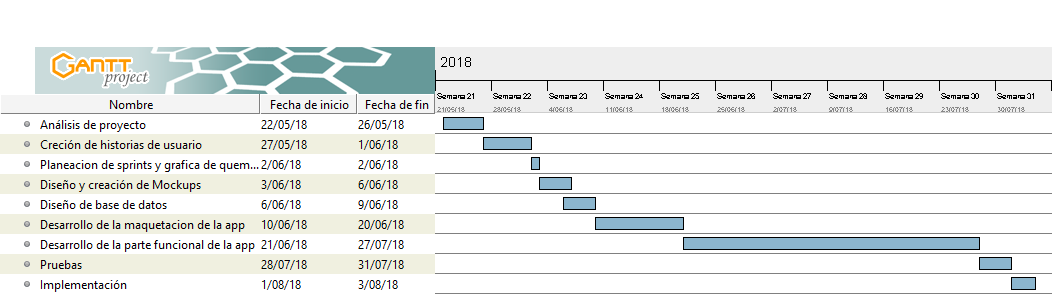
\includegraphics[scale=0.6]{img/cronograma.png} 
		\caption{Cronograma de actividades a seguir.}
		\label{gantt}
	\end{center}
\end{figure}

\section{Encuesta}
Se realizó una encuesta a los alumnos de la carrera de Ingenieria en Software del 3° cutatrimestre de la Universidad Politecnica de Pachuca, con el fin de que con los resultados poder formular las historias de usuario. Se obtuvieron los siguientes resultados:

\begin{figure}[H]
	\begin{center}
		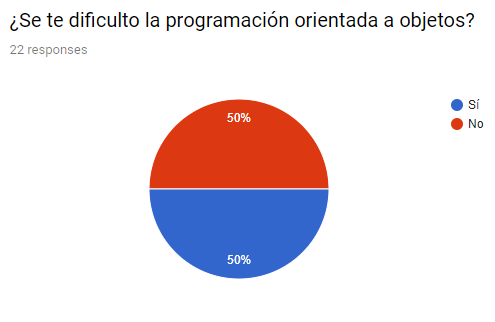
\includegraphics[scale=0.6]{img/pregunta1.png} 
		\caption{Primera pregunta de la encuesta..}
		\label{p1}
	\end{center}
\end{figure}
En la primera pregunta se puede observar que a un 50\% de los alumnos de les dificulta la programación orientada a objetos, mientras que al 50\% restante no se le dificulta.

\begin{figure}[H]
	\begin{center}
		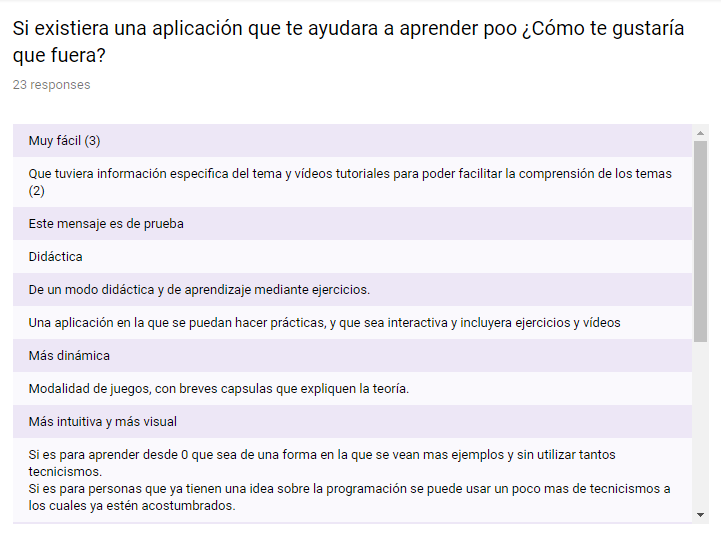
\includegraphics[scale=0.6]{img/pregunta21} 
		\caption{Segunda pregunta del cuestionario (parte 1).}
		\label{p21}
	\end{center}
\end{figure}
\begin{figure}[H]
	\begin{center}
		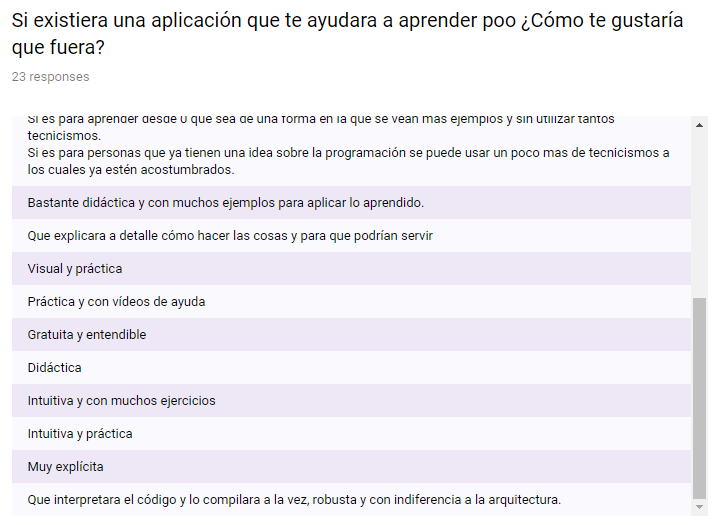
\includegraphics[scale=0.6]{img/pregunta22} 
		\caption{Segunda pregunta del cuestionario (parte 2).}
		\label{p22}
	\end{center}
\end{figure}
En la segunda pregunta, tres alumnos respondiéron que la aplicación fuera "muy facil," mientras que dos alumnos respondieron que la aplicación contuviera información muy especifica del tema y tutoriales para facilitar la comprensión del tema, mientras que los demás alumnos respondieron con respuestas como que sea didactica, dinámica, intuitiva, con una modadlidad de juegos, que no contenga muchos tecnisismos y con videos de ayuda.

\begin{figure}[H]
	\begin{center}
		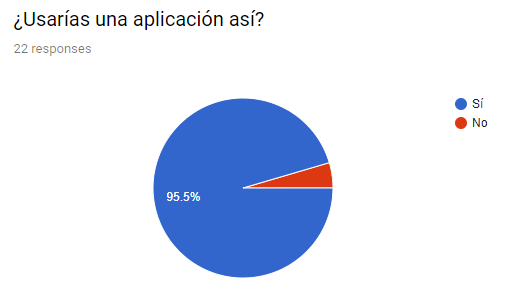
\includegraphics[scale=0.6]{img/pregunta3.png} 
		\caption{Tercera pregunta del cuestionario.}
		\label{p3}
	\end{center}
\end{figure}
En la tercera pregunta del cuestionario, el 95.5\% de los alumnos repondieron aafirmativamente a que si utilizarían una aplicación de acuerdo a lo que respondieron anteriormente, mientras que el 4.5\% restante respondio de forma negativa.

\section{Historias de usuario}

\begin{table}[H]\small
\begin{tabular}{@{\extracolsep{\fill}} | p{5cm} | p{5cm} | p{5cm} | }
\multicolumn{3}{|c|}{1. Aplicación didactica} \\ \hline
  \hline
\multicolumn{3}{|p{15cm}|}{Como usuario quisiera que la aplicación fuera de un modo didáctica y de aprendizaje mediante ejercicios.} \\ \hline
\hline
Estimaci'on: 7 &semanas	Valor: 50	& Dependencias: \\
\hline
\multicolumn{3}{|p{15cm}|}{Condiciones de satisfacci'on:
\begin{itemize}
	\item La aplicación contendrá información selecta y bien explicada.
	\item Se incluirán algunos ejercicios los cuales deberán resolverse en la computadora.
\end{itemize}
}\\ \hline
\hline
\end{tabular}
\caption{Historia de usuario 1}
\label{hu1}
\end{table}
%%%%%%%%%%%%%%%%%%%%%%%%%%%%%%%%%%%%%%%%%%%%%%%%%%%%%%%%%%%%%%%%%%%%%%%%%%%%%%%%%%%%%%
\begin{table}[H]\small
\begin{tabular}{@{\extracolsep{\fill}} | p{5cm} | p{5cm} | p{5cm} | }
\multicolumn{3}{|c|}{2. Explicaciónes detalladas} \\ \hline
  \hline
\multicolumn{3}{|p{15cm}|}{Como usuario quisiera que explicara a detalle cómo hacer las cosas y para que podrían servir.} \\ \hline
\hline
Estimaci'on: 7 &semanas	Valor: 60	& Dependencias: \\
\hline
\multicolumn{3}{|p{15cm}|}{Condiciones de satisfacci'on:
\begin{itemize}
	\item Se dará una aplicación detallada de cada tema así como ejemplos de uso.
\end{itemize}
}\\ \hline
\hline
\end{tabular}
\caption{Historia de usuario 2}
\label{hu2}
\end{table}
%%%%%%%%%%%%%%%%%%%%%%%%%%%%%%%%%%%%%%%%%%%%%%%%%%%%%%%%%%%%%%%%%%%%%%%%%%%%%%%%%%%%%%
\begin{table}[H]\small
\begin{tabular}{@{\extracolsep{\fill}} | p{5cm} | p{5cm} | p{5cm} | }
\multicolumn{3}{|c|}{3. Modalidad de juegos} \\ \hline
  \hline
\multicolumn{3}{|p{15cm}|}{Como usuario quisiera que la aplicación tuviera la modalidad de juegos, con breves capsulas que expliquen la teoría.} \\ \hline
\hline
Estimaci'on: 6 &semanas	Valor: 60	& Dependencias: \\
\hline
\multicolumn{3}{|p{15cm}|}{Condiciones de satisfacci'on:
\begin{itemize}
	\item Se pondrá información sobre algunos conceptos y se hará un pequeño test de manera que ayude a recordar.
\end{itemize}
}\\ \hline
\hline
\end{tabular}
\caption{Historia de usuario 3}
\label{hu3}
\end{table}
%%%%%%%%%%%%%%%%%%%%%%%%%%%%%%%%%%%%%%%%%%%%%%%%%%%%%%%%%%%%%%%%%%%%%%%%%%%%%%%%%%%%%%
\begin{table}[H]\small
\begin{tabular}{@{\extracolsep{\fill}} | p{5cm} | p{5cm} | p{5cm} | }
\multicolumn{3}{|c|}{4. Información especifica} \\ \hline
  \hline
\multicolumn{3}{|p{15cm}|}{Como usuario quisiera que tuviera información específica del tema y vídeos tutoriales para poder facilitar la comprensión de los temas.} \\ \hline
\hline
Estimaci'on: 6 &semanas	Valor: 30	& Dependencias: \\
\hline
\multicolumn{3}{|p{15cm}|}{Condiciones de satisfacci'on:
\begin{itemize}
	\item Se dará la información de manera específica pero en lugar de videos se incluirán algunos ejemplos.
\end{itemize}
}\\ \hline
\hline
\end{tabular}
\caption{Historia de usuario 4}
\label{hu4}
\end{table}
%%%%%%%%%%%%%%%%%%%%%%%%%%%%%%%%%%%%%%%%%%%%%%%%%%%%%%%%%%%%%%%%%%%%%%%%%%%%%%%%%%%%%%
\begin{table}[H]\small
\begin{tabular}{@{\extracolsep{\fill}} | p{5cm} | p{5cm} | p{5cm} | }
\multicolumn{3}{|c|}{5. Visual y practica} \\ \hline
  \hline
\multicolumn{3}{|p{15cm}|}{Como usuario quisiera que la aplicación fuera visual y práctica.} \\ \hline
\hline
Estimaci'on: 4 &semanas	Valor: 20	& Dependencias: \\
\hline
\multicolumn{3}{|p{15cm}|}{Condiciones de satisfacci'on:
\begin{itemize}
	\item La aplicación será visual y de fácil utilización.
\end{itemize}
}\\ \hline
\hline
\end{tabular}
\caption{Historia de usuario 5}
\label{hu5}
\end{table}
%%%%%%%%%%%%%%%%%%%%%%%%%%%%%%%%%%%%%%%%%%%%%%%%%%%%%%%%%%%%%%%%%%%%%%%%%%%%%%%%%%%%%%
\begin{table}[H]\small
\begin{tabular}{@{\extracolsep{\fill}} | p{5cm} | p{5cm} | p{5cm} | }
\multicolumn{3}{|c|}{6. Intuitiva} \\ \hline
  \hline
\multicolumn{3}{|p{15cm}|}{Como usuario quisiera que la aplicación fuera intuitiva y con muchos ejercicios.} \\ \hline
\hline
Estimaci'on: 3 &semanas	Valor: 20	& Dependencias: \\
\hline
\multicolumn{3}{|p{15cm}|}{Condiciones de satisfacci'on:
\begin{itemize}
	\item Se creará una interfaz amigable con el usuario y fácil de aprender.
\end{itemize}
}\\ \hline
\hline
\end{tabular}
\caption{Historia de usuario 6}
\label{hu6}
\end{table}
%%%%%%%%%%%%%%%%%%%%%%%%%%%%%%%%%%%%%%%%%%%%%%%%%%%%%%%%%%%%%%%%%%%%%%%%%%%%%%%%%%%%%%
\begin{table}[H]\small
\begin{tabular}{@{\extracolsep{\fill}} | p{5cm} | p{5cm} | p{5cm} | }
\multicolumn{3}{|c|}{7. Con ejemplos y pocos tecnicismos } \\ \hline
  \hline
\multicolumn{3}{|p{15cm}|}{Como usuario quisiera que si es para aprender desde 0 que sea de una forma en la que se vean más ejemplos y sin hacer uso excesivo de tecnicismos.} \\ \hline
\hline
Estimaci'on: 3 &semanas	Valor: 20	& Dependencias: \\
\hline
\multicolumn{3}{|p{15cm}|}{Condiciones de satisfacci'on:
\begin{itemize}
	\item Se intentará utilizar pocas palabras técnicas, más sin embargo estas irán apareciendo para que después el usuario las pueda entender.
	\item Se incluirán varios ejemplos y ejercicios.
\end{itemize}
}\\ \hline
\hline
\end{tabular}
\caption{Historia de usuario 7}
\label{hu7}
\end{table}

\section{Grafica de quemado}
\begin{figure}[H]
	\begin{center}
		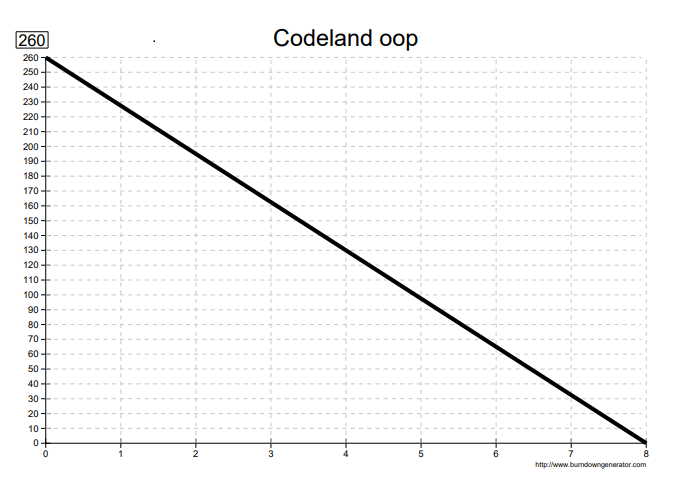
\includegraphics[scale=0.7]{img/quemado.png} 
		\caption{Grafica de quemado de las historias de usuario.}
		\label{quemado}
	\end{center}
\end{figure}

\section{Maquetado}
\begin{figure}[H]
\begin{center}
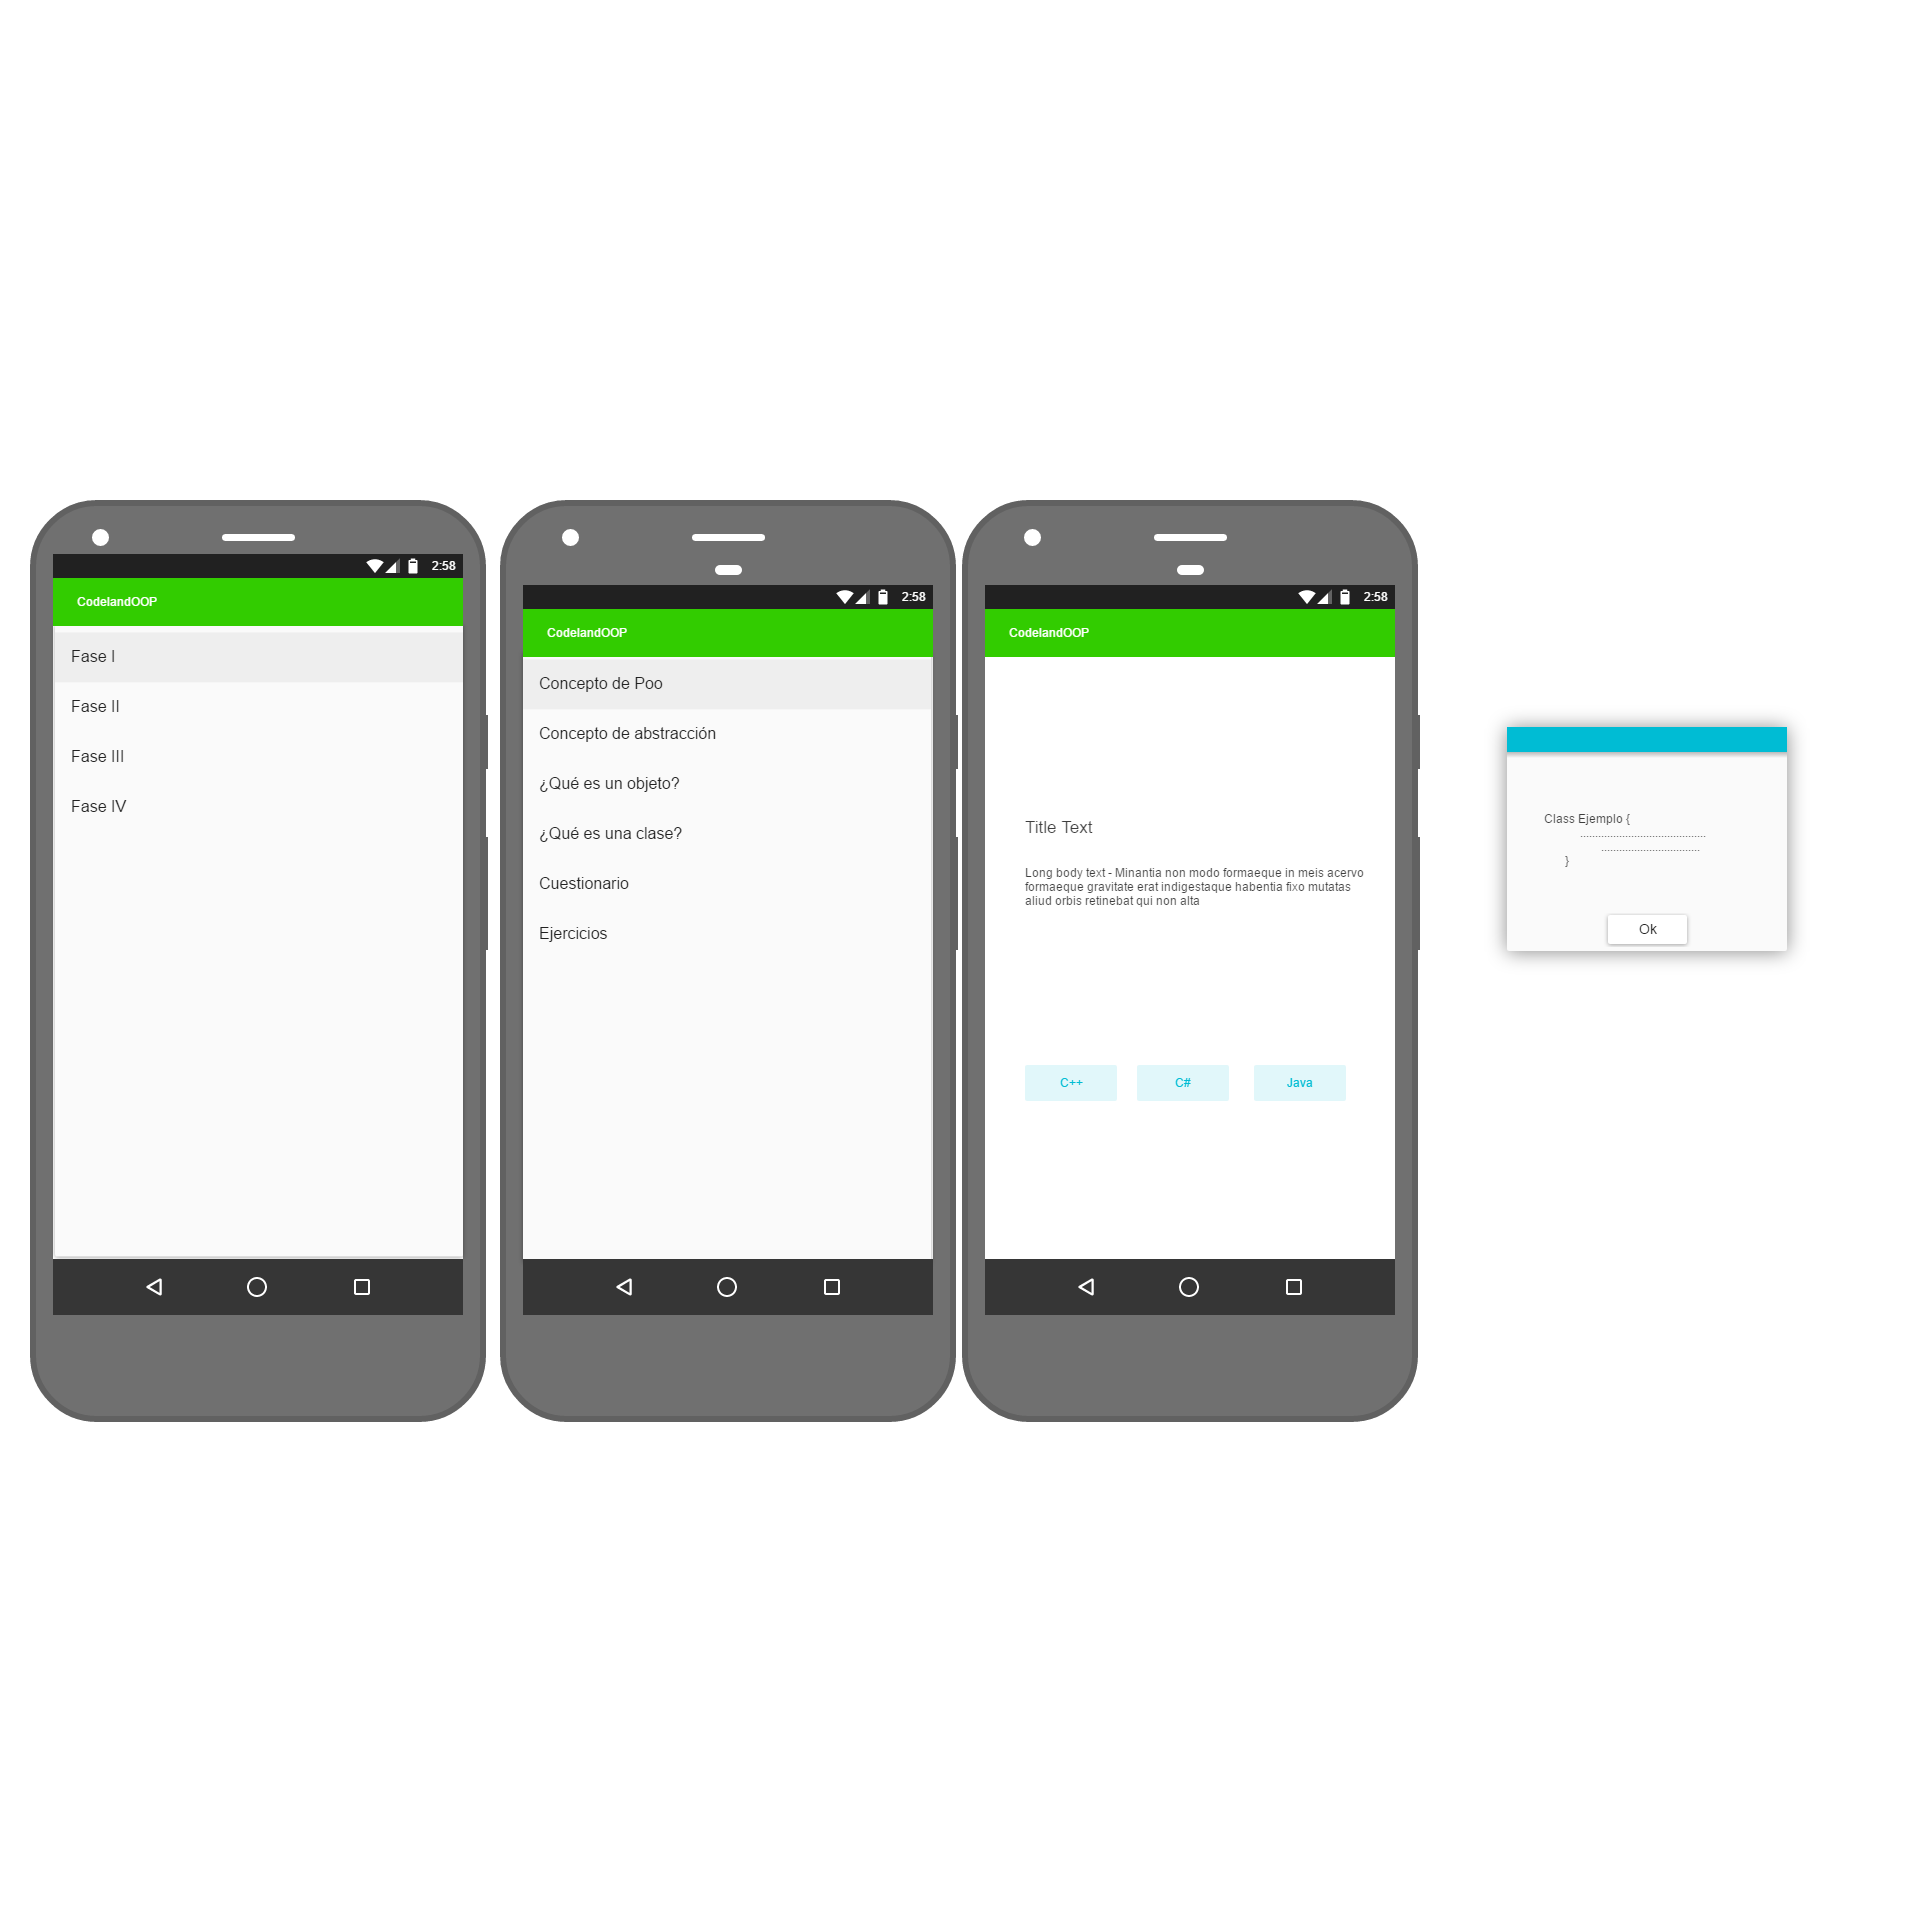
\includegraphics[scale=0.2]{img/pantallas1.png} 
\end{center}
\caption{Pantallas de las fases, temas, tema, ejercicios y ejemplo.}
\end{figure}


